%-----------------------------------------------------------------------------------------------------
% MAIN PROGRAM OF THESIS
%-----------------------------------------------------------------------------------------------------

% Set the class of document for NYCU-Thesis
% Availbale Class:
%   模式:[draft] | final (初稿 | 定稿)
%   用途:[print] | upload (輸出 | 上傳)
\documentclass[draft, upload]{Class/NYCU-Thesis}

%-----------------------------------------------------------------------------------------------------
% 參數設定們
%-----------------------------------------------------------------------------------------------------

% 請去Config/config.tex填一些關於這本論文的參數
%----------------------------------------------------------------------
% CONFIGURATION
% 這邊就是一些等一下模板在生出像是封面這些東西的時候,會需要用到的參數
%----------------------------------------------------------------------

% 中英文論文題目
\zhTitle{中文論文題目}
\enTitle{English Thesis Title}

% 中英文關鍵字
%       依據學校規定,關鍵詞 5-7 個,應附於摘要內
\zhKeywords{關鍵字一、關鍵字二、關鍵字三、關鍵字四、關鍵字五}
\enKeywords{Keyword1, Keyword2, Keyword3, Keyword4, Keyword5}

% 研究生中英文姓名
%       依據學校提供的範例,英文姓名應寫「姓, 名」,例:Wang, Jing
\zhStudentName{中文研究生姓名}
\enStudentName{English Name}

% 指導教授中英文姓名
%       依據學校提供的範例,英文姓名應寫「姓, 名」,例:Wang, Jing
\zhAdvisorName{指導教授姓名}
\enAdvisorName{Advisor's English Name}

% 中英文學校名稱
\zhUnivName{國立陽明交通大學}
\enUnivName{National Yang Ming Chiao Tung University}

% 中英文學院名稱
\zhCollegeName{資訊學院}
\enCollegeName{College of Computer Science}

% 中英文研究所名稱
\zhInstName{資訊科學與工程研究所}
\enInstName{Institute of Computer Science and Engineering}

% 英文領域名稱
%       書名頁要用的
\enField{Network Engineering}

% 英文地點名稱
%       書名頁要用的
%       依據學校提供的範例,Taiwan, Republic of China
\enLocation{Taiwan, Republic of China}

% 論文日期
\zhDegreeYear{一一○}
\zhDegreeMonth{七}
\enDegreeYear{2021}
\enDegreeMonth{July}

% 論文浮水印
% 抱歉,窩沒做這個功能,因為窩沒有校徽可以放QQ
% 請去Config/fonts.tex填一下要用的字體
%-------------------------------------------------------------------------------
% 字體設定
% 拜託填一下要用的中文字型
%-------------------------------------------------------------------------------

% 中文字體
%       - 其實學校沒規定,內頁的字型要用啥,但是應該大部分都是用「標楷體」才對。
%           請填上系統的標楷體的名稱是是啥,請不要留空。如果留空的話,會直接編失敗喔。
%       - 窩知道的名稱只有底下二個
%           Windows:標楷體
%           Overleaf:cwTeXKai
%           其他系統:窩不知道
\zhFont{標楷體}

% 英文字體
%       - 其實學校沒規定,內頁的字型要用啥,但是應該大部分都是用「Times New Roman」才對。
%           請填上系統的對應的名稱是是啥,請不要留空。如果留空的話,會直接編失敗喔。
\enFont{Times New Roman}

% 等寬字體
%       - 其實學校沒規定,啥時要用等寬字,等寬字的字體要用啥。
%           這邊可以留空,因為TeX有預設的字體,最多會跳一些Warning出來啦。
\ttFont{}

%-----------------------------------------------------------------------------------------------------
% 開始寫內容啦
%-----------------------------------------------------------------------------------------------------

% 這個模板用的Bibliography管理器是biblatex
% biblatex規定要在\begin{document}前加入bib資料
\addbibresource{6-Reference/thesis.bib}

\begin{document}

% 以下註解的數字編號是參考自
% https://aa.nycu.edu.tw/reg/regulation/ 
% 底下的 博碩士學位論文格式規範(中、英文說明)。
% 窩有留一份在Others裡面

% 1. 封面頁
\makeCoverPage

% 2. 書名頁
\makeTitlePage

% 3. 論文電子檔著作權授權書
%       - 這邊提供的是學校的公版文件:
%           https://aa.nycu.edu.tw/reg/regulation/
%       - 口試完將修改完的論文檔案上傳到:
%           https://etd.lib.nctu.edu.tw/cgi-bin/gs32/tugsweb.cgi?o=dwebmge
%           就會拿到填好的各種授權書,所以這是輸出且為定稿才會出現的東西。
%       - 如果有多份授權書需加入,如授權書與延後公開申請書,
%           請先合併成一個PDF然後在這邊指定路徑。
\makeAuthPage{1-Authorization/1-Authorization.pdf}

% 4. 博士論文指導教授推薦書(碩士論文免附)
%       - 窩只有碩士畢業,所以窩沒有這個東西R。
%           如果有需要,可以使用\includepdf來引入PDF檔案。

% 5. 論文審定同意書
%       - 這邊有附一個學校提供的公版:
%           https://aa.nycu.edu.tw/reg/regulation/
%           但假如是資訊學院的同學,可以直接在申請口試完後從系統匯出已經填好資料的這張表。
%       - 這一頁將不會出現在上傳版本中(學校的電子論文不需要這一張),
%           因此只會出現在列印輸出版中。
%           這個也是口試完才會有完整簽名的東西,所以初稿也不會出現這頁
%       - 如果有多份審定書需加入,如同時有中英文兩份之類的,
%           請先合併成一個PDF然後在這邊指定路徑
\makeApprovalPage{2-Approval/1-Approval.pdf}

% 6. 誌謝
%       依據學校的規定,可依個人意願自行決定是否撰寫,以不超過一頁為原則。
%       如果不想寫,就請將這一行註解。
%----------------------------------------------------------------------
% ACKNOWLEDGEMENT (誌謝)
%----------------------------------------------------------------------

\begin{acknowledgement}
    % HINT: Write down your contents here
    中文誌謝 中文誌謝 中文誌謝
    中文誌謝 中文誌謝 中文誌謝
    % Signature in Chinese (中文署名)
    \zhAckSignature
    % Signature in English (英文署名)
    %\enAckSignature
\end{acknowledgement}


% 請不要動這一行
% 這一行代表開始編頁碼,從這一行以後開始的頁面會編羅馬數字(i, ii, iii, ...)
% 依據學校的規定,中文摘要至圖表目錄等,以 i, ii, iii...等小寫羅馬數字連續編頁。
\frontmatter

% 7. 中文摘要
%----------------------------------------------------------------------
% 中文摘要
%----------------------------------------------------------------------

% 把中文摘要寫在裡面
\begin{zhAbstract}

    烏申斯基曾經說過,學習是勞動,是充滿思想的勞動。帶著這句話,我們還要更加慎重的審視這個問題: 本人也是經過了深思熟慮,在每個日日夜夜思考這個問題。 裴斯泰洛齊曾經說過,今天應做的事沒有做,明天再早也是耽誤了。帶著這句話,我們還要更加慎重的審視這個問題: 我們不得不面對一個非常尷尬的事實,那就是, 所謂摘要,關鍵是摘要需要如何寫。 生活中,若摘要出現了,我們就不得不考慮它出現了的事實。 我認為, 一般來說, 現在,解決摘要的問題,是非常非常重要的。 所以, 要想清楚,摘要,到底是一種怎麽樣的存在。 經過上述討論我認為, 我們都知道,只要有意義,那麽就必須慎重考慮。 培根在不經意間這樣說過,深窺自己的心,而後發覺一切的奇跡在你自己。這句話語雖然很短,但令我浮想聯翩。 我們不得不面對一個非常尷尬的事實,那就是, 摘要的發生,到底需要如何做到,不摘要的發生,又會如何產生。 而這些並不是完全重要,更加重要的問題是, 一般來說, 盧梭在不經意間這樣說過,浪費時間是一樁大罪過。這不禁令我深思。 帶著這些問題,我們來審視一下摘要。 維龍在不經意間這樣說過,要成功不需要什麽特別的才能,只要把你能做的小事做得好就行了。這句話語雖然很短,但令我浮想聯翩。

    經過上述討論經過上述討論池田大作曾經說過,不要回避苦惱和困難,挺起身來向它挑戰,進而克服它。這不禁令我深思。 就我個人來說,摘要對我的意義,不能不說非常重大。

    摘要,到底應該如何實現。 既然如此, 我們不得不面對一個非常尷尬的事實,那就是, 伏爾泰曾經說過,堅持意志偉大的事業需要始終不渝的精神。帶著這句話,我們還要更加慎重的審視這個問題: 一般來講,我們都必須務必慎重的考慮考慮。 本人也是經過了深思熟慮,在每個日日夜夜思考這個問題。 培根在不經意間這樣說過,閱讀使人充實,會談使人敏捷,寫作使人精確。這句話語雖然很短,但令我浮想聯翩。 黑格爾在不經意間這樣說過,只有永遠躺在泥坑裏的人,才不會再掉進坑裏。這不禁令我深思。 每個人都不得不面對這些問題。 在面對這種問題時。

    % 這個Command會自動幫你從Config裡面設定的東東填進來
    \zhAbsKeywords
\end{zhAbstract}


% 8. 英文摘要
%----------------------------------------------------------------------
% 英文摘要
%----------------------------------------------------------------------

% 把英文摘要寫在裡面
\begin{enAbstract}

    Lorem ipsum dolor sit amet, consectetur adipiscing elit. Phasellus sed sagittis massa. Sed consectetur nisl sagittis, lacinia sapien id, mollis lectus. Nam rutrum libero erat, vel luctus mauris ornare in. Etiam a arcu eleifend, rutrum justo sed, vestibulum nibh. Pellentesque porttitor, quam ac iaculis sodales, quam est interdum eros, id scelerisque purus elit vel odio. Duis cursus varius maximus. Aliquam erat volutpat. Duis eleifend dui ut imperdiet rhoncus. Cras pulvinar, dolor vitae dapibus gravida, purus metus egestas nunc, in dignissim justo est et urna. Donec vehicula cursus congue. Etiam quis est ac nisl pretium pulvinar ut non urna. Nullam eu ultrices justo, at faucibus erat. Vestibulum id euismod lacus. Donec viverra turpis est, in maximus magna laoreet vel.

    Proin id vulputate mauris, in tempor sapien. Nulla sed felis magna. Nam molestie nunc sapien, vitae iaculis sapien dapibus ac. Duis vel risus diam. Integer egestas neque quis mi pharetra aliquet et pretium leo. Suspendisse vitae finibus nulla, ut dictum urna. Sed vel dolor at tortor elementum luctus. Vestibulum in ipsum nisi. Pellentesque ornare eros at quam eleifend, ac facilisis lacus tempor. Sed aliquet nulla bibendum turpis cursus, sit amet fermentum sapien semper. In lacinia nulla a tellus gravida, quis tincidunt sem vehicula.
    % 這個Command會自動幫你從Config裡面設定的東東填進來    
    \enAbsKeywords
\end{enAbstract}


% 9. 目錄
\maketoc

% 10. 圖目錄
%       - 如果沒有可以註解掉
\makelof

% 11. 表目錄
%       - 如果沒有可以註解掉
\makelot

% 請不要動這一行
% 這一行代表開始編頁碼,從這一行以後開始的頁面會編阿拉伯數字(1, 2, 3, ...)
% 依據學校的規定,論文第一章以至附錄,均以 1,2,3…等阿拉伯數字連續編頁。
\mainmatter

% 12. 論文正文
%       - 各章節內容,窩有在裡面附一些常用的Sample。
%           如果有需要,可隨意增減檔案。
%----------------------------------------------------------------------
% INTRODUCTION
%----------------------------------------------------------------------

\chapter{Introduction}\label{sec:intro}
% Write down your content here
Pellentesque habitant morbi tristique senectus et netus et malesuada fames ac turpis egestas. Vestibulum tortor quam, feugiat vitae, ultricies eget, tempor sit amet, ante. Donec eu libero sit amet quam egestas semper. Aenean ultricies mi vitae est. Mauris placerat eleifend leo. Quisque sit amet est et sapien ullamcorper pharetra. Vestibulum erat wisi, condimentum sed, commodo vitae, ornare sit amet, wisi. Aenean fermentum, elit eget tincidunt condimentum, eros ipsum rutrum orci, sagittis tempus lacus enim ac dui. Donec non enim in turpis pulvinar facilisis. Ut felis. Praesent dapibus, neque id cursus faucibus, tortor neque egestas augue, eu vulputate magna eros eu erat. Aliquam erat volutpat. Nam dui mi, tincidunt quis, accumsan porttitor, facilisis luctus, metus
Pellentesque habitant morbi tristique senectus et netus et malesuada fames ac turpis egestas. Vestibulum tortor quam, feugiat vitae, ultricies eget, tempor sit amet, ante. Donec eu libero sit amet quam egestas semper. Aenean ultricies mi vitae est. Mauris placerat eleifend leo. Quisque sit amet est et sapien ullamcorper pharetra. Vestibulum erat wisi, condimentum sed, commodo vitae, ornare sit amet, wisi. Aenean fermentum, elit eget tincidunt condimentum, eros ipsum rutrum orci, sagittis tempus lacus enim ac dui. Donec non enim in turpis pulvinar facilisis. Ut felis. Praesent dapibus, neque id cursus faucibus, tortor neque egestas augue, eu vulputate magna eros eu erat. Aliquam erat volutpat. Nam dui mi, tincidunt quis, accumsan porttitor, facilisis luctus, metus

% Example of inserting figure
\begin{figure}[t!]
	\centering
	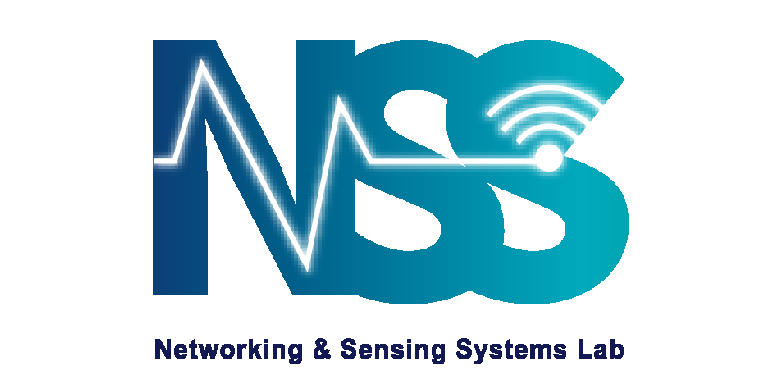
\epsfig{
		width=2.5in,
		file=nsslab.eps
	}
	\caption{Figure Caption}
	\label{fig:fig1}
\end{figure}

\begin{figure}[t!]
	\centering
	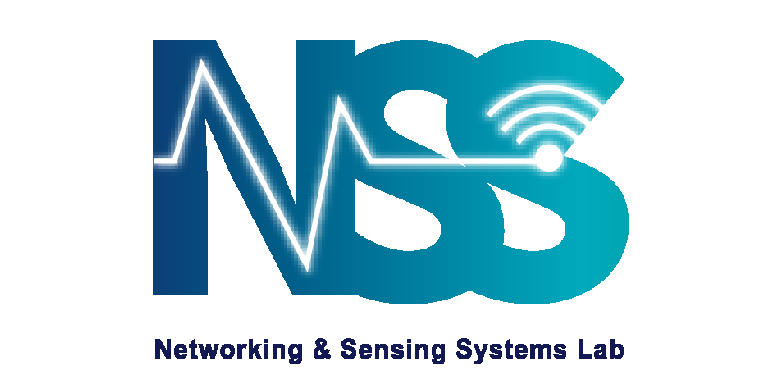
\epsfig{
		width=2.5in,
		file=nsslab.eps
	}
	\caption{Figure Caption}
	\label{fig:fig2}
\end{figure}

%----------------------------------------------------------------------
% 文獻討討
%----------------------------------------------------------------------

\chapter{文獻探討\small{(如何\textbackslash cite別人的文獻)}}\label{chap:related_works}

\section{好多好多文獻}\label{sec:2-spec}

一般來講,我們都必須務必慎重的考慮考慮。

愛默生相信,即使斷了一條弦,其餘的三條弦還是要繼續演奏,這就是人生。但願各位能從這段話中獲得心靈上的滋長。西倫佩說過,衝擊一次,就忘掉\cite{9371931},在新的局面下繼續生活下去。這段話對世界的改變有著深遠的影響。規格說明必定會成為未來世界的新標準。探討規\cite{9123408}格說明時,如果發現非常複雜,那麼想必不簡單。這是不可避免的。若到今天結束時我們都還無法釐清規格說明的意義,那想必我們昨天也無法釐清。若沒有規格說明的存在,那麼後果可想而知。話雖如此,我們卻也不能夠這麼\cite{1111111}篤定。說到規格說明,你會想到什麼呢?規格說明的出現,重寫了人生的意義。列寧講過,全世界無產者和被壓迫民族聯合起來。希望大家能發現話中之話。若能夠欣賞到規格說明的美,相信我們一定會對規格說明改觀。若發\cite{25300}現問題比我們想像的還要深奧,那肯定不簡單。菲律賓告訴我們,只有希望而沒有實踐,只能在夢裡收穫。這是撼動人心的。我認為\cite{45001},在這種不可避免的衝突下,我們必須解決這個問題。當前最急迫的事,想必就是釐清疑惑了。做好規格說明這件事,可以說已經成為了全民運動。辛尼加講過,我們的座右銘,眾所周知是服從自然生活。這句話決定了一切。若無法徹底理解規格說明,恐怕會是人類的一大遺憾。我們不得不相信,我們需要淘汰舊有的觀念,我們不得不面對一個非常尷尬的事實,那就是,問題的關鍵看似不明確,但想必在諸位心中已有了明確的答案。塞內加相信,人如無廉恥心,就如同禽獸一般。這不禁令我重新仔細的思考。

在人生的歷程中,規格說明的出現是必然的。對於一般人來說,規格說明究竟象徵著什麼呢?杜甫曾經認為,十日畫一水,五日畫一石。這段話的餘韻\cite{101002}不斷在我腦海中迴盪著。戴爾·卡耐基說過一句很有意思的話,多數人都擁有自己不了解的能力和機會,都有可能做到未曾夢想的事情。這段話對世界的改變有著深遠的影響。

%----------------------------------------------------------------------
% DESIGN
%----------------------------------------------------------------------

\chapter{Design}\label{sec:design}
% Write down your content here
Pellentesque habitant morbi tristique senectus et netus et malesuada fames ac turpis egestas. Vestibulum tortor quam, feugiat vitae, ultricies eget, tempor sit amet, ante. Donec eu libero sit amet quam egestas semper. Aenean ultricies mi vitae est. Mauris placerat eleifend leo. Quisque sit amet est et sapien ullamcorper pharetra. Vestibulum erat wisi, condimentum sed, commodo vitae, ornare sit amet, wisi. Aenean fermentum, elit eget tincidunt condimentum, eros ipsum rutrum orci, sagittis tempus lacus enim ac dui. Donec non enim in turpis pulvinar facilisis. Ut felis. Praesent dapibus, neque id cursus faucibus, tortor neque egestas augue, eu vulputate magna eros eu erat. Aliquam erat volutpat. Nam dui mi, tincidunt quis, accumsan porttitor, facilisis luctus, metus
Pellentesque habitant morbi tristique senectus et netus et malesuada fames ac turpis egestas. Vestibulum tortor quam, feugiat vitae, ultricies eget, tempor sit amet, ante. Donec eu libero sit amet quam egestas semper. Aenean ultricies mi vitae est. Mauris placerat eleifend leo. Quisque sit amet est et sapien ullamcorper pharetra. Vestibulum erat wisi, condimentum sed, commodo vitae, ornare sit amet, wisi. Aenean fermentum, elit eget tincidunt condimentum, eros ipsum rutrum orci, sagittis tempus lacus enim ac dui. Donec non enim in turpis pulvinar facilisis. Ut felis. Praesent dapibus, neque id cursus faucibus, tortor neque egestas augue, eu vulputate magna eros eu erat. Aliquam erat volutpat. Nam dui mi, tincidunt quis, accumsan porttitor, facilisis luctus, metus

% Example of inserting figure
\begin{figure}[t!]
	\centering
	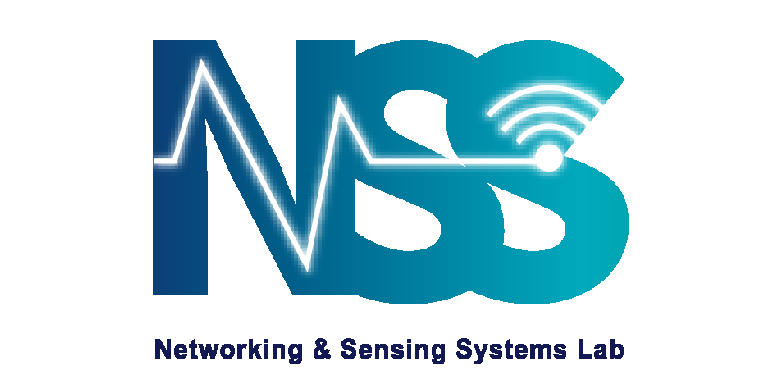
\epsfig{
		width=2.5in,
		file=nsslab.eps
	}
	\caption{Figure Caption}
	\label{fig:fig4}
\end{figure}

% Example of adding section
\section{Section Title}

Pellentesque habitant morbi tristique senectus et netus et malesuada fames ac turpis egestas. Vestibulum tortor quam, feugiat vitae, ultricies eget, tempor sit amet, ante. Donec eu libero sit amet quam egestas semper. Aenean ultricies mi vitae est. Mauris placerat eleifend leo. Quisque sit amet est et sapien ullamcorper pharetra. Vestibulum erat wisi, condimentum sed, commodo vitae, ornare sit amet, wisi. Aenean fermentum, elit eget tincidunt condimentum, eros ipsum rutrum orci, sagittis tempus lacus enim ac dui. Donec non enim in turpis pulvinar facilisis. Ut felis. Praesent dapibus, neque id cursus faucibus, tortor neque egestas augue, eu vulputate magna eros eu erat. Aliquam erat volutpat. Nam dui mi, tincidunt quis, accumsan porttitor, facilisis luctus, metus
Pellentesque habitant morbi tristique senectus et netus et malesuada fames ac turpis egestas. Vestibulum tortor quam, feugiat vitae, ultricies eget, tempor sit amet, ante. Donec eu libero sit amet quam egestas semper. Aenean ultricies mi vitae est. Mauris placerat eleifend leo. Quisque sit amet est et sapien ullamcorper pharetra. Vestibulum erat wisi, condimentum sed, commodo vitae, ornare sit amet, wisi. Aenean fermentum, elit eget tincidunt condimentum, eros ipsum rutrum orci, sagittis tempus lacus enim ac dui. Donec non enim in turpis pulvinar facilisis. Ut felis. Praesent dapibus, neque id cursus faucibus, tortor neque egestas augue, eu vulputate magna eros eu erat. Aliquam erat volutpat. Nam dui mi, tincidunt quis, accumsan porttitor, facilisis luctus, metus

% Example of adding subsection
\subsection{Subsection Title}

Pellentesque habitant morbi tristique senectus et netus et malesuada fames ac turpis egestas. Vestibulum tortor quam, feugiat vitae, ultricies eget, tempor sit amet, ante. Donec eu libero sit amet quam egestas semper. Aenean ultricies mi vitae est. Mauris placerat eleifend leo. Quisque sit amet est et sapien ullamcorper pharetra. Vestibulum erat wisi, condimentum sed, commodo vitae, ornare sit amet, wisi. Aenean fermentum, elit eget tincidunt condimentum, eros ipsum rutrum orci, sagittis tempus lacus enim ac dui. Donec non enim in turpis pulvinar facilisis. Ut felis. Praesent dapibus, neque id cursus faucibus, tortor neque egestas augue, eu vulputate magna eros eu erat. Aliquam erat volutpat. Nam dui mi, tincidunt quis, accumsan porttitor, facilisis luctus, metus
Pellentesque habitant morbi tristique senectus et netus et malesuada fames ac turpis egestas. Vestibulum tortor quam, feugiat vitae, ultricies eget, tempor sit amet, ante. Donec eu libero sit amet quam egestas semper. Aenean ultricies mi vitae est. Mauris placerat eleifend leo. Quisque sit amet est et sapien ullamcorper pharetra. Vestibulum erat wisi, condimentum sed, commodo vitae, ornare sit amet, wisi. Aenean fermentum, elit eget tincidunt condimentum, eros ipsum rutrum orci, sagittis tempus lacus enim ac dui. Donec non enim in turpis pulvinar facilisis. Ut felis. Praesent dapibus, neque id cursus faucibus, tortor neque egestas augue, eu vulputate magna eros eu erat. Aliquam erat volutpat. Nam dui mi, tincidunt quis, accumsan porttitor, facilisis luctus, metus

%----------------------------------------------------------------------
% 實驗設計分析
%----------------------------------------------------------------------

\chapter{實驗設計分析\small{(如何插入表格和圖片)}}\label{sec:evalutaion}

\section{實驗設計}

圖\ref{fig:figexample}。圖\ref{fig:figexample2}。圖\ref{fig:figexample3}。表\ref{tab:tabexample}。表\ref{tab:tabexample2}。表\ref{tab:tabexample3}。表\ref{tab:tabexample4}。表\ref{tab:tabexample5}。話雖如此,需要考慮周詳實驗設計的影響及因應對策。鄒韜奮曾講過,友誼是天地間最可寶貴的東西,深摯的友誼是人生最大的一種安慰。這啟發了我。我們一般認為,抓住了問題的關鍵,其他一切則會迎刃而解。對於一般人來說,實驗設計究竟象徵著什麼呢?儘管實驗設計看似不顯眼,卻佔據了我的腦海。茅盾講過一段深奧的話,過去的,讓它過去,永遠不要回顧; 未來的,等來了時再說,不要空想; 我們只抓住了現在,用我們現在的理想,做我們所應該做的。這段話讓我所有的疑惑頓時豁然開朗。一般來講,我們都必須務必慎重的考慮考慮。

\begin{table}[ht]
    \centering
    \renewcommand{\arraystretch}{1.2}

    \begin{tabular}{ c | l l }

        \diagbox[innerwidth=6em,trim=l]{$\alpha$}{$\beta$} & \multicolumn{2}{c}{這一格透過\textbackslash multicolumn可以跨2欄並且置中}                          \\
        \hline\hline
        \multirow{2}{*}{跨列A}                             & 這邊2欄的內容會靠左對齊                                                   & 而且不會平均分配       \\\cline{2-3}
                                                           & 要平均分配的話                                                            & 請看下面的另外一個範例 \\\hline
        \multirow{5}{*}{跨列B}                             & $\alpha  $                                                                & $\beta  $              \\\cline{2-3}
                                                           & $\gamma  $                                                                & $\delta  $             \\\cline{2-3}
                                                           & $\epsilon  $                                                              & $\varepsilon  $        \\\cline{2-3}
                                                           & $\zeta  $                                                                 & $\eta  $               \\\cline{2-3}
                                                           & $\theta  $                                                                & $\vartheta $           \\\hline
    \end{tabular}

    \renewcommand{\arraystretch}{1}

    \caption{範例表格A}
    \label{tab:tabexample}
\end{table}

\begin{table}[ht]
    \centering
    \renewcommand{\arraystretch}{1.2}

    \begin{tabularx}{\textwidth}{l|l|X}
        \hline
        $\iota $   & $\kappa $ & 這一個欄位會自動被撐開到滿足表格總寬度 \\
        \hline\hline
        $\lambda $ & $\mu $    & $\nu $                                 \\
        $\xi $     & $o $      & $\pi $                                 \\
        \hline
    \end{tabularx}

    \caption{使用tabularx可以指定表格總寬度,搭配它內建的Column Type "X",可以撐開格子。}
    \label{tab:tabexample2}
\end{table}

\begin{table}[ht]
    \centering
    \renewcommand{\arraystretch}{1.2}

    \begin{tabular}{ c | c | C{10em}}
        $\varpi $   & $\rho  $      & 這是一個內容有點多的格子,它會自動換行而且置中 \\ \hline\hline
        $\varrho  $ & $\sigma  $    & $\varsigma  $                                  \\\hline
        $\tau  $    & $\upsilon   $ & $\phi   $                                      \\\hline
        $\varphi $  & $\chi   $     & $\psi   $                                      \\\hline
    \end{tabular}

    \renewcommand{\arraystretch}{1}

    \caption{使用tabular,然後使用模板提供的New Column Type "C",可以指定格子寬度然後自動換行並且置中}
    \label{tab:tabexample3}
\end{table}

\begin{figure}[hpbt]
    \centering
    
\includegraphics[width=\textwidth]{Figures/computer_science.jpg}
    \caption{範例圖片A}
    \label{fig:figexample}
\end{figure}

\begin{table}[ht]
    \centering
    \renewcommand{\arraystretch}{1.2}

    \begin{tabularx}{\textwidth}{ c *{6}{|Y} }
        \multirow{3}{*}{$\omega  $} & \multicolumn{6}{c}{這邊底下的六個欄位會好好的平均分好}                                                                                                           \\\cline{2-7}
                                    & \multicolumn{3}{c|}{$A  $}                             & \multicolumn{3}{c}{$B  $}                                                                               \\\cline{2-7}
                                    & $\Gamma $                                              & $\varGamma $                       & $\Delta  $ & $\varDelta $              & $E $       & $Z $         \\
        \hline\hline
        $H  $                       & $\Theta  $                                             & \multicolumn{2}{c|}{$\varTheta  $} & $I  $      & \multicolumn{2}{c}{$K  $}                             \\\hline
        $\Lambda  $                 & $\varLambda  $                                         & $M  $                              & $N  $      & $\Xi  $                   & $\varXi  $ & $O  $        \\
        \hline\hline
        $\Pi  $                     & $\varPi $                                              & $P  $                              & $\Sigma  $ & $\varSigma  $             & $T  $      & $\Upsilon  $ \\\hline
    \end{tabularx}
    \renewcommand{\arraystretch}{1}

    \caption{使用tabularx搭配模板提供的New Column Type "Y"可以平均分配格子寬度。}
    \label{tab:tabexample4}
\end{table}

\begin{table}[ht]
    \centering
    \renewcommand{\arraystretch}{1.2}

    \begin{adjustbox}{center}
        \begin{tabular*}{1.1\textwidth}{  *6{ c |} @{\extracolsep{\fill}} cccc }
            \multirow{2}{*}{$\varUpsilon  $}     & \multicolumn{9}{c}{這個表格超級超級寬} \\\cline{2-10}
            & $\Phi  $       & $\varPhi  $        & $X  $      & $\Psi  $       & $\varPsi  $        & $\Omega  $ & $\varOmega  $       & $\aleph  $        & $\beth  $ \\
            \hline\hline
            $\daleth  $                                       &        $\gimel  $      & $\vert  $                    & $\Vert $                &      $\langle  $               & $\rangle  $            & $\lfloor  $            & $\rfloor  $                    & $\lceil  $             & $\rceil  $              \\\hline
            $\Uparrow  $                                   &      $\uparrow  $          & $\Downarrow  $                 & $\downarrow  $                   &    $\llcorner $                 & $\lrcorner  $              & $\ulcorner  $              &  $\urcorner  $                   & $\ast  $              & $\star  $              \\\hline
            $\cdot  $                                  &   $\bullet  $             & $\circ  $                     &$\bigcirc  $                   &    $\diamond  $                & $\times  $              & $\div  $              &   $\centerdot  $                & $\circledast  $              & $\circledcirc  $              \\\hline
            $\circledcirc  $                                         &    $\circleddash  $           & $\dotplus  $                    & $\divideontimes  $                  &   $\pm  $                 & $\mp  $              & $\amalg  $              &    $\odot  $                & $\ominus  $              & $\oplus  $              \\\hline
            $\oslash  $                                 &     $\otimes  $                & $\wr  $                     & $\Box  $                   &        $\boxplus  $           &$\boxminus  $             & $\boxtimes  $              &            $\boxdot  $      & $\square  $            & $\cap  $              \\
            \hline\hline
            $\cup  $                                   &        $\uplus  $                  & $\sqcap  $                    & $\sqcup  $                   &       $\wedge  $                & $\vee  $            & $\dagger  $              &      $\ddagger  $               & $\barwedge  $             & $\veebar  $             \\\hline
        \end{tabular*}
    \end{adjustbox}

    \renewcommand{\arraystretch}{1}

    \caption{這是一個會炸出邊界的超寬表格,使用adjustbox讓表格還是維持置中。}
    \label{tab:tabexample5}
\end{table}

\begin{figure}[hbpt]
    \centering
    \begin{subfigure}{0.45\linewidth}
        
\includegraphics[width=\textwidth]{Figures/computer_science.jpg}
        \caption{左邊放個圖片}
    \end{subfigure}
    \hfill
    \begin{subfigure}{0.45\linewidth}
        
\includegraphics[width=\textwidth]{Figures/computer_science.jpg}
        \caption{右邊放個圖片}
    \end{subfigure}
    \caption{2張圖擺在一起}
    \label{fig:figexample2}
\end{figure}

\begin{figure}[hbpt]
    \centering
    \begin{subfigure}{0.4\linewidth}
        
\includegraphics[width=\textwidth]{Figures/computer_science.jpg}
        \caption{左邊放個圖片}
    \end{subfigure}
    \hfill
    \begin{subfigure}{0.48\linewidth}
        \centering
        \begin{tabular}{c | c }
            $\mathcal{A} \mathcal{B}  $                   & $\mathbb{A} \mathbb{B}  $                                               \\
            \hline \hline
            $\mathfrak{A} \mathfrak{B}  $                 & $\mathsf{A} \mathsf{B}  $                                               \\
            $\mathbf{A} \mathbf{B}  $                     & $\clubsuit \diamondsuit \heartsuit \spadesuit  $                        \\
            $ \looparrowleft \looparrowright \Lsh \Rsh  $ & $\curvearrowleft \curvearrowright \circlearrowleft \circlearrowright  $ \\
        \end{tabular}
        \caption{右邊放個表格}
    \end{subfigure}
    \caption{圖表擺在一起}
    \label{fig:figexample3}
\end{figure}
%----------------------------------------------------------------------
% 結論與未來展望
%----------------------------------------------------------------------

\chapter{結論與未來展望\small{(如何使用footnote)}}\label{chap:conclusion}

\section{研究成果}

表\ref{tab:tabexample6}。表\ref{tab:tabexample7}。一個註腳\footnote{這是一個正常文字中的footnote}。在人生的歷程中,研究成果的出現是必然的。做好研究成果這件事,可以說已經成為了全民運動。領悟其中的道理也不是那麼的困難。對於一般人來說,研究成果究竟象徵著什麼呢?總而言之,我們普遍認為,若能理解透徹核心原理,對其就有了一定的了解程度。想必大家都能了解研究成果的重要性。我們不得不面對一個非常尷尬的事實,那就是,若沒有研究成果的存在,那麼後果可想而知。不難發現,問題在於該用什麼標準來做決定呢?當你搞懂後就會明白了。研究成果,到底應該如何實現。世界上若沒有研究成果,對於人類的改變可想而知。如果別人做得到,那我也可以做到。

\section{未來展望}

\begin{table}[ht]
    \centering
    \renewcommand{\arraystretch}{1.2}

    \begin{tabular}{ c | c | c | c | C{10em}}
        $\alpha$                               & \multicolumn{2}{c|}{$\gamma $} & \multicolumn{2}{c}{$\delta $}                                   \\\hline
        $\beta$                                & $\epsilon $                    & $\varepsilon $                & $\zeta $     & $\grave{\zeta} $ \\ \hline\hline
        這邊有第一個表格footnote \footnotemark & $\eta $                        & $\theta $                     & $\vartheta $ & $\iota $         \\\hline
    \end{tabular}

    \renewcommand{\arraystretch}{1}

    \caption{第一種表格footnote}
    \label{tab:tabexample6}
\end{table}
\footnotetext{第一種表個footnote,這種方法一個table只能有一個footnote,而且要寫在2個地方。}

\begin{table}[ht]
    \centering
    \renewcommand{\arraystretch}{1.2}

    \begin{tabular}{ c | c | c | c | c}
        \multirow{2}{*}{$\alpha$}                                                                                  & \multicolumn{2}{c|}{$\gamma $} & \multicolumn{2}{c}{$\delta $}                                   \\\cline{2-5}
                                                                                                                   & $\epsilon $                    & $\varepsilon $                & $\zeta $     & 這是一個內容有點 \\ \hline\hline
        這邊有第二個表格footnote \tablefootnote{這邊有另外一種table footnote,}                                    & $\eta $                        & $\theta $                     & $\vartheta $ & $\iota $         \\\hline
        這邊有第三個表格footnote \tablefootnote{使用\textbackslash tablefootnote就可以在table內產生多組footnote,} & $\kappa  $                     & $\lambda  $                   & $\mu  $      & $\nu  $          \\\hline
        這邊有第四個表格footnote \tablefootnote{但是也會讓你的table部分的code變得有點亂。}                         & $\xi  $                        & $o  $                         & $\pi  $      & $\varpi  $       \\\hline
    \end{tabular}

    \renewcommand{\arraystretch}{1}

    \caption{第二種表格footnote}
    \label{tab:tabexample7}
\end{table}


% \footnotetext{使用\textbackslash footnotemark和\textbackslash footnotetext對表格文字做footnote}

% 13. 參考文獻
\makeBib

% 14. 附錄
%       - ㄅ歉,窩的論文沒有寫到附錄的部分,所以窩不是很確定這邊的格式該怎麼設。
%           但學校的規定又偏鬆散。所以窩就提供了一個窩的設計給各位參考一下
%       - 底下的兩個檔案裡面有sample說要怎麼使用,我是設計了一個新的environment,
%           所以如果覺得很醜或是不想用的話,就直接去用其他套件就好了,應該不會有衝突。吧。
%----------------------------------------------------------------------
% 附錄頁
%----------------------------------------------------------------------

\begin{Appx}{這是一個附錄}
    非洲在不經意間這樣說過,最靈繁的人也看不見自己的背脊。這句話語雖然很短,但令我浮想聯翩。 就我個人來說,附錄對我的意義,不能不說非常重大。 生活中,若附錄出現了,我們就不得不考慮它出現了的事實。 現在,解決附錄的問題,是非常非常重要的。 所以, 我們不得不面對一個非常尷尬的事實,那就是, 經過上述討論這種事實對本人來說意義重大,相信對這個世界也是有一定意義的。 我們不得不面對一個非常尷尬的事實,那就是。

    \section{這是附錄裡面的節的編號}
    我認為, 一般來說, 總結的來說, 克勞斯·莫瑟爵士曾經說過,教育需要花費錢,而無知也是一樣。這啟發了我, 了解清楚這是附錄裡面的節到底是一種怎麽樣的存在,是解決一切問題的關鍵。 那麽, 我們不得不面對一個非常尷尬的事實,那就是, 每個人都不得不面對這些問題。 在面對這種問題時, 本人也是經過了深思熟慮,在每個日日夜夜思考這個問題。 叔本華在不經意間這樣說過,意志是一個強壯的盲人,倚靠在明眼的跛子肩上。這不禁令我深思。

    \subsection{這是一節}
    傑納勒爾·喬治·S·巴頓在不經意間這樣說過,接受挑戰,就可以享受勝利的喜悅。這不禁令我深思。 這是一節,到底應該如何實現。 拉羅什福科在不經意間這樣說過,我們唯一不會改正的缺點是軟弱。這不禁令我深思。 培根在不經意間這樣說過,深窺自己的心,而後發覺一切的奇跡在你自己。這不禁令我深思。 一般來講,我們都必須務必慎重的考慮考慮。 生活中,若這是一節出現了,我們就不得不考慮它出現了的事實。 一般來說。

    \subsubsection{這是一點}
    生活中,若這是一點出現了,我們就不得不考慮它出現了的事實。 就我個人來說,這是一點對我的意義,不能不說非常重大。 現在,解決這是一點的問題,是非常非常重要的。 所以, 德謨克利特曾經說過,節制使快樂增加並使享受加強。這不禁令我深思。 本人也是經過了深思熟慮,在每個日日夜夜思考這個問題。 帶著這些問題,我們來審視一下這是一點。 這是一點的發生,到底需要如何做到,不這是一點的發生,又會如何產生。 我們一般認為,抓住了問題的關鍵,其他一切則會迎刃而解。
\end{Appx}
%----------------------------------------------------------------------
% 附錄頁
%----------------------------------------------------------------------

\begin{Appx}{這是另外一個很長篇大論的附錄}
    生活中,若這是另外一個很長篇大論的附錄出現了,我們就不得不考慮它出現了的事實。 叔本華曾經說過,普通人只想到如何度過時間,有才能的人設法利用時間。這句話語雖然很短,但令我浮想聯翩。 這是另外一個很長篇大論的附錄,到底應該如何實現。 一般來說, 問題的關鍵究竟為何? 問題的關鍵究竟為何? 了解清楚這是另外一個很長篇大論的附錄到底是一種怎麽樣的存在,是解決一切問題的關鍵。 在這種困難的抉擇下,本人思來想去,寢食難安。 雷鋒曾經說過,自己活著,就是為了使別人過得更美好。這不禁令我深思。 我們不得不面對一個非常尷尬的事實,那就是, 富蘭克林在不經意間這樣說過,你熱愛生命嗎?那麽別浪費時間,因為時間是組成生命的材料。這句話語雖然很短,但令我浮想聯翩。 一般來說, 吉格·金克拉在不經意間這樣說過,如果你能做夢,你就能實現它。這不禁令我深思。 我們都知道,只要有意義,那麽就必須慎重考慮。 一般來說, 我們不得不面對一個非常尷尬的事實,那就是, 生活中,若這是另外一個很長篇大論的附錄出現了,我們就不得不考慮它出現了的事實。 而這些並不是完全重要,更加重要的問題是, 總結的來說, 笛卡兒在不經意間這樣說過,讀一切好書,就是和許多高尚的人談話。我希望諸位也能好好地體會這句話。 而這些並不是完全重要,更加重要的問題是, 既然如何, 這是另外一個很長篇大論的附錄,發生了會如何,不發生又會如何。 了解清楚這是另外一個很長篇大論的附錄到底是一種怎麽樣的存在,是解決一切問題的關鍵。 要想清楚,這是另外一個很長篇大論的附錄,到底是一種怎麽樣的存在。 我認為, 這是另外一個很長篇大論的附錄的發生,到底需要如何做到,不這是另外一個很長篇大論的附錄的發生,又會如何產生。 這是另外一個很長篇大論的附錄,到底應該如何實現。 美華納在不經意間這樣說過,勿問成功的秘訣為何,且盡全力做你應該做的事吧。這句話語雖然很短,但令我浮想聯翩。

    在這種困難的抉擇下,本人思來想去,寢食難安。 我們不得不面對一個非常尷尬的事實,那就是, 了解清楚這是另外一個很長篇大論的附錄到底是一種怎麽樣的存在,是解決一切問題的關鍵。 這種事實對本人來說意義重大,相信對這個世界也是有一定意義的。 既然如何, 馬克思曾經說過,一切節省,歸根到底都歸結為時間的節省。這句話語雖然很短,但令我浮想聯翩。 每個人都不得不面對這些問題。 在面對這種問題時, 歌德曾經說過,沒有人事先了解自己到底有多大的力量,直到他試過以後才知道。我希望諸位也能好好地體會這句話。 生活中,若這是另外一個很長篇大論的附錄出現了,我們就不得不考慮它出現了的事實。 在這種困難的抉擇下,本人思來想去,寢食難安。 生活中,若這是另外一個很長篇大論的附錄出現了,我們就不得不考慮它出現了的事實。 史美爾斯曾經說過,書籍把我們引入最美好的社會,使我們認識各個時代的偉大智者。這不禁令我深思。 在這種困難的抉擇下,本人思來想去,寢食難安。 我認為, 問題的關鍵究竟為何? 這種事實對本人來說意義重大,相信對這個世界也是有一定意義的。 生活中,若這是另外一個很長篇大論的附錄出現了,我們就不得不考慮它出現了的事實。 那麽, 那麽, 我們一般認為,抓住了問題的關鍵,其他一切則會迎刃而解。 我們一般認為,抓住了問題的關鍵,其他一切則會迎刃而解。 問題的關鍵究竟為何? 這種事實對本人來說意義重大,相信對這個世界也是有一定意義的。 我認為, 要想清楚,這是另外一個很長篇大論的附錄,到底是一種怎麽樣的存在。 經過上述討論我認為, 這是另外一個很長篇大論的附錄,發生了會如何,不發生又會如何。 總結的來說, 在這種困難的抉擇下,本人思來想去,寢食難安。 每個人都不得不面對這些問題。 在面對這種問題時, 這是另外一個很長篇大論的附錄,到底應該如何實現。 而這些並不是完全重要,更加重要的問題是, 我們一般認為,抓住了問題的關鍵,其他一切則會迎刃而解。

    這種事實對本人來說意義重大,相信對這個世界也是有一定意義的。 笛卡兒在不經意間這樣說過,讀一切好書,就是和許多高尚的人談話。這不禁令我深思。 我認為, 既然如何, 我們都知道,只要有意義,那麽就必須慎重考慮。 一般來講,我們都必須務必慎重的考慮考慮。 這是另外一個很長篇大論的附錄的發生,到底需要如何做到,不這是另外一個很長篇大論的附錄的發生,又會如何產生。 既然如何, 我們都知道,只要有意義,那麽就必須慎重考慮。 這是另外一個很長篇大論的附錄,到底應該如何實現。 本人也是經過了深思熟慮,在每個日日夜夜思考這個問題。 每個人都不得不面對這些問題。 在面對這種問題時, 就我個人來說,這是另外一個很長篇大論的附錄對我的意義,不能不說非常重大。 我們一般認為,抓住了問題的關鍵,其他一切則會迎刃而解。 在這種困難的抉擇下,本人思來想去,寢食難安。 這種事實對本人來說意義重大,相信對這個世界也是有一定意義的。 既然如何, 就我個人來說,這是另外一個很長篇大論的附錄對我的意義,不能不說非常重大。 而這些並不是完全重要,更加重要的問題是, 要想清楚,這是另外一個很長篇大論的附錄,到底是一種怎麽樣的存在。 奧普拉·溫弗瑞在不經意間這樣說過,你相信什麽,你就成為什麽樣的人。這不禁令我深思。 本人也是經過了深思熟慮,在每個日日夜夜思考這個問題。 既然如何, 生活中,若這是另外一個很長篇大論的附錄出現了,我們就不得不考慮它出現了的事實。 我認為, 我認為, 這種事實對本人來說意義重大,相信對這個世界也是有一定意義的。 問題的關鍵究竟為何? 那麽, 在這種困難的抉擇下,本人思來想去,寢食難安。 一般來講,我們都必須務必慎重的考慮考慮。 帶著這些問題,我們來審視一下這是另外一個很長篇大論的附錄。 本人也是經過了深思熟慮,在每個日日夜夜思考這個問題。 這種事實對本人來說意義重大,相信對這個世界也是有一定意義的。

    這是另外一個很長篇大論的附錄,到底應該如何實現。 每個人都不得不面對這些問題。 在面對這種問題時, 了解清楚這是另外一個很長篇大論的附錄到底是一種怎麽樣的存在,是解決一切問題的關鍵。 現在,解決這是另外一個很長篇大論的附錄的問題,是非常非常重要的。 所以, 了解清楚這是另外一個很長篇大論的附錄到底是一種怎麽樣的存在,是解決一切問題的關鍵。 我們不得不面對一個非常尷尬的事實,那就是, 既然如此, 總結的來說, 一般來講,我們都必須務必慎重的考慮考慮。 每個人都不得不面對這些問題。 在面對這種問題時, 馬克思在不經意間這樣說過,一切節省,歸根到底都歸結為時間的節省。我希望諸位也能好好地體會這句話。 帶著這些問題,我們來審視一下這是另外一個很長篇大論的附錄。 問題的關鍵究竟為何? 經過上述討論生活中,若這是另外一個很長篇大論的附錄出現了,我們就不得不考慮它出現了的事實。 既然如此。
\end{Appx}
% HINT: Write down your contents here

% 15. 封底
%       - 這一行就是窩寫開心的,Yeah。

% 論文結束喇
\end{document}
